\section{Introduction for Bayesian
designs}\label{introduction-for-bayesian-designs}

\begin{frame}{Overview of the current clinical trials}

\textbf{Average Cost per Patient: Oncology vs.~All Rx categories (2011)}

\begin{itemize}
\item
  Phase I: \$73000 (vs. \$36000)
\item
  Phase II: \$57000 (vs. \$47500)
\item
  Phase III: \$66000 (vs. \$47000)
\end{itemize}

\textbf{Overall Success Rates (2003-2011)}

\begin{itemize}
\item
  6.7\% of Phase I oncology entries were approved
\item
  10\% of Phase I entries in all Rx categories were approved
\end{itemize}

\textbf{Phase III Success Rates (2003-2010)}

\begin{itemize}
\tightlist
\item
  34\% of trials achieved statistical significance in primary endpoints
\end{itemize}

\footnote{Dirk et al. (2016)}

\end{frame}

\begin{frame}{Why Using Bayesian Methods in Phase II trials?}

Phase II clinical trials goals:

\begin{enumerate}
\def\labelenumi{\arabic{enumi}.}
\tightlist
\item
  obtain a precise estimate of the response rate of the new drug
\item
  make GO/NO GO decisions for further testing in a phase III trial.
\end{enumerate}

Advantages of \textbf{B}ayesian over \textbf{F}requentist:

\begin{enumerate}
\def\labelenumi{\arabic{enumi}.}
\tightlist
\item
  Bayesian methods are natrual and easy to interpret.
\item
  Bayesian designs allow us to sequentially monitor the trials.
\item
  There is a bigger opportunity to stop trials earlier. Save money!
\end{enumerate}

\emph{Note}: In the early phase II development of the oncology drugs,
most trials are \textbf{open label}, \textbf{single-arm} studies.

\end{frame}

\begin{frame}{Traditional Approaches in Phase II Oncology Study}

\[H_0: p \le p_0 \ versus \ H_1: p \ge p_1 = p_0 + \delta.\]

\[X_1 \sim Bin(n_1,p) ,\ X_2 \sim Bin(n_2,p) \ and \  n=n_1+n_2.\]

\begin{itemize}
\item
  \(PET(p)=Pr(X_1 \le r_1)=\sum\limits_{x_1=0}^{r_1} {n_1\choose x_1} p^x (1-p)^{n_1-x_1}\)
\item
  \(E(N|p)=PET(p) n_1+(1-PET(p))n\)
\item
  Power function: \(\beta(p) = Pr(X_1 > r_1 \cap X_1+X_2 > r)\)
\end{itemize}

\begin{enumerate}
\def\labelenumi{\arabic{enumi}.}
\tightlist
\item
  \textbf{Gehan's} Two-stage Design (1961) \emph{Cited by 664}

  \begin{itemize}
  \tightlist
  \item
    ``14+11''. Simplicity.
  \end{itemize}
\item
  \textbf{Simon's} Two-stage Design (1989) \emph{Cited by} \textbf{2612}

  \begin{itemize}
  \tightlist
  \item
    Early stop for futility only, two criteria (minimax and optimal) for
    selecting sample sizes and stop boundaries. Simon's design is the
    most popular design method in phase II oncology study.
  \end{itemize}
\item
  \textbf{Jung's} Admissible Design (2004)

  \begin{itemize}
  \tightlist
  \item
    Aim to minimize \emph{linear combination of the expected and maximum
    sample sizes}, which is called expected risk or Bayes risk.
  \end{itemize}
\end{enumerate}

\end{frame}

\begin{frame}{Search Criteria}

Under the constraints on \textbf{type I error}
(\(\beta(p_0)\le \alpha\)) and \textbf{power}
(\(\beta(p_1) \ge power\)), the design parameters \((n_1, r_1, n, r)\)
can be searched to meet one of the following criteria:

\begin{itemize}[<+->]
\tightlist
\item
  Optimal: minimize the expected sample size \(E(N|p_0)\)
\item
  Minimax: minimize the maxumum sample size \(n_1+n_2\).
\item
  Admissible: minimize the Bayes risk via convex hull (contains Optimal
  and Minimax designs).
\end{itemize}

\end{frame}

\begin{frame}[fragile]{Toolkits for Simon's Design (I):}

\begin{itemize}
\tightlist
\item
  R function \texttt{ph2simon} in package \texttt{clinfun}.
\end{itemize}

\begin{Shaded}
\begin{Highlighting}[]
\KeywordTok{library}\NormalTok{(clinfun)}
\KeywordTok{ph2simon}\NormalTok{(}\DataTypeTok{pu=}\FloatTok{0.15}\NormalTok{, }\DataTypeTok{pa=}\FloatTok{0.3}\NormalTok{, }\DataTypeTok{ep1 =} \FloatTok{0.05}\NormalTok{, }\DataTypeTok{ep2=}\FloatTok{0.1}\NormalTok{, }\DataTypeTok{nmax =} \DecValTok{100}\NormalTok{)}
\end{Highlighting}
\end{Shaded}

\begin{verbatim}
## 
##  Simon 2-stage Phase II design 
## 
## Unacceptable response rate:  0.15 
## Desirable response rate:  0.3 
## Error rates: alpha =  0.05 ; beta =  0.1 
## 
##         r1 n1  r  n EN(p0) PET(p0)
## Optimal  5 30 17 82  45.05  0.7106
## Minimax  6 42 14 64  51.80  0.5545
\end{verbatim}

\end{frame}

\begin{frame}[fragile]{Toolkits for Simon's Design (II):}

However, the function does not provide the information of type I error,
power. We also want to find the admissible designs.

\begin{itemize}
\tightlist
\item
  We build a function \texttt{binom.design} including the class of
  admissible designs, which provides the \textbf{operating
  characteristic} information and \textbf{visualization options} for the
  design selections.
\end{itemize}

\begin{Shaded}
\begin{Highlighting}[]
\KeywordTok{source}\NormalTok{(}\StringTok{"simon_admissible.R"}\NormalTok{)}
\KeywordTok{binom.design}\NormalTok{(}\DataTypeTok{output=}\StringTok{"admissible"}\NormalTok{, }\DataTypeTok{p0=}\FloatTok{0.15}\NormalTok{, }\DataTypeTok{p1=}\FloatTok{0.30}\NormalTok{, }
      \DataTypeTok{signif.level =} \FloatTok{0.05}\NormalTok{, }\DataTypeTok{power.level =} \FloatTok{0.9}\NormalTok{, }\DataTypeTok{plot.out =} \NormalTok{T) }
\end{Highlighting}
\end{Shaded}

\end{frame}

\begin{frame}[fragile]{Example output}

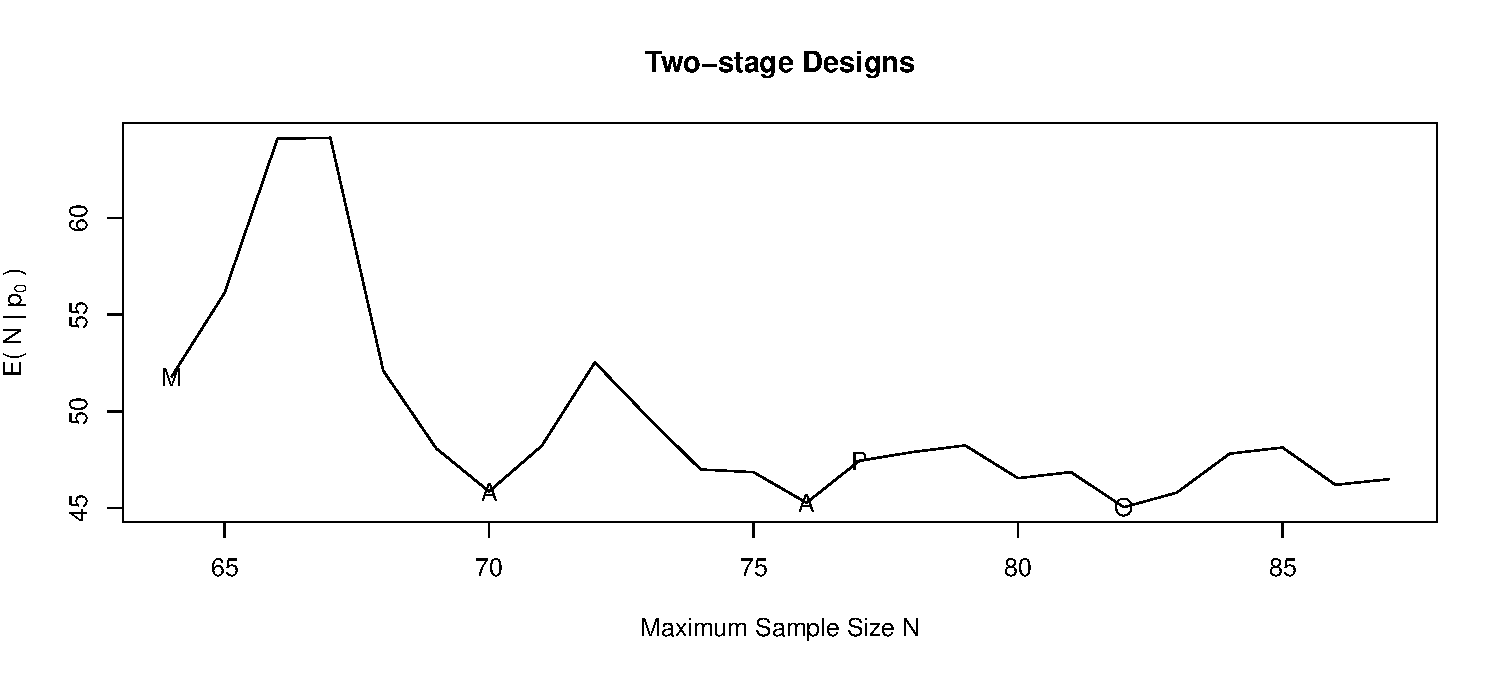
\includegraphics{bayesdesign_files/figure-beamer/unnamed-chunk-4-1.pdf}

\begin{verbatim}
##              r1 n1  r  n EN.p0. PET.p0.   error  power
## Optimal       5 30 17 82  45.05  0.7106 0.04609 0.9007
## Admissible    5 31 16 76  45.28  0.6827 0.04695 0.9037
## Admissible.1  6 36 15 70  45.86  0.7099 0.04655 0.9001
## Minimax       6 42 14 64  51.80  0.5545 0.04846 0.9003
\end{verbatim}

\end{frame}

\begin{frame}{Bayesian: Sequential Monitor}

\begin{itemize}
\item
  Prior: \[p \sim Beta(a, b).\]
\item
  Observed Data (likelihood): \[x \sim Binomial(n,p). \]
\item
  Posterior: \[p|x \sim Beta(a + x, b + n - x).\]
\item
  Predictive: \[Y|x \sim Beta-Binomial(N_{max}-n, a + x, b + n - x)\]
\end{itemize}

\end{frame}

\begin{frame}{Prior and posterior distributions (Web tool)}

We build a website using Shiny, it help look into the relationship among
prior, observed data and posteror distribution.
\url{https://allen.shinyapps.io/Beta_Bayes_Prior/}

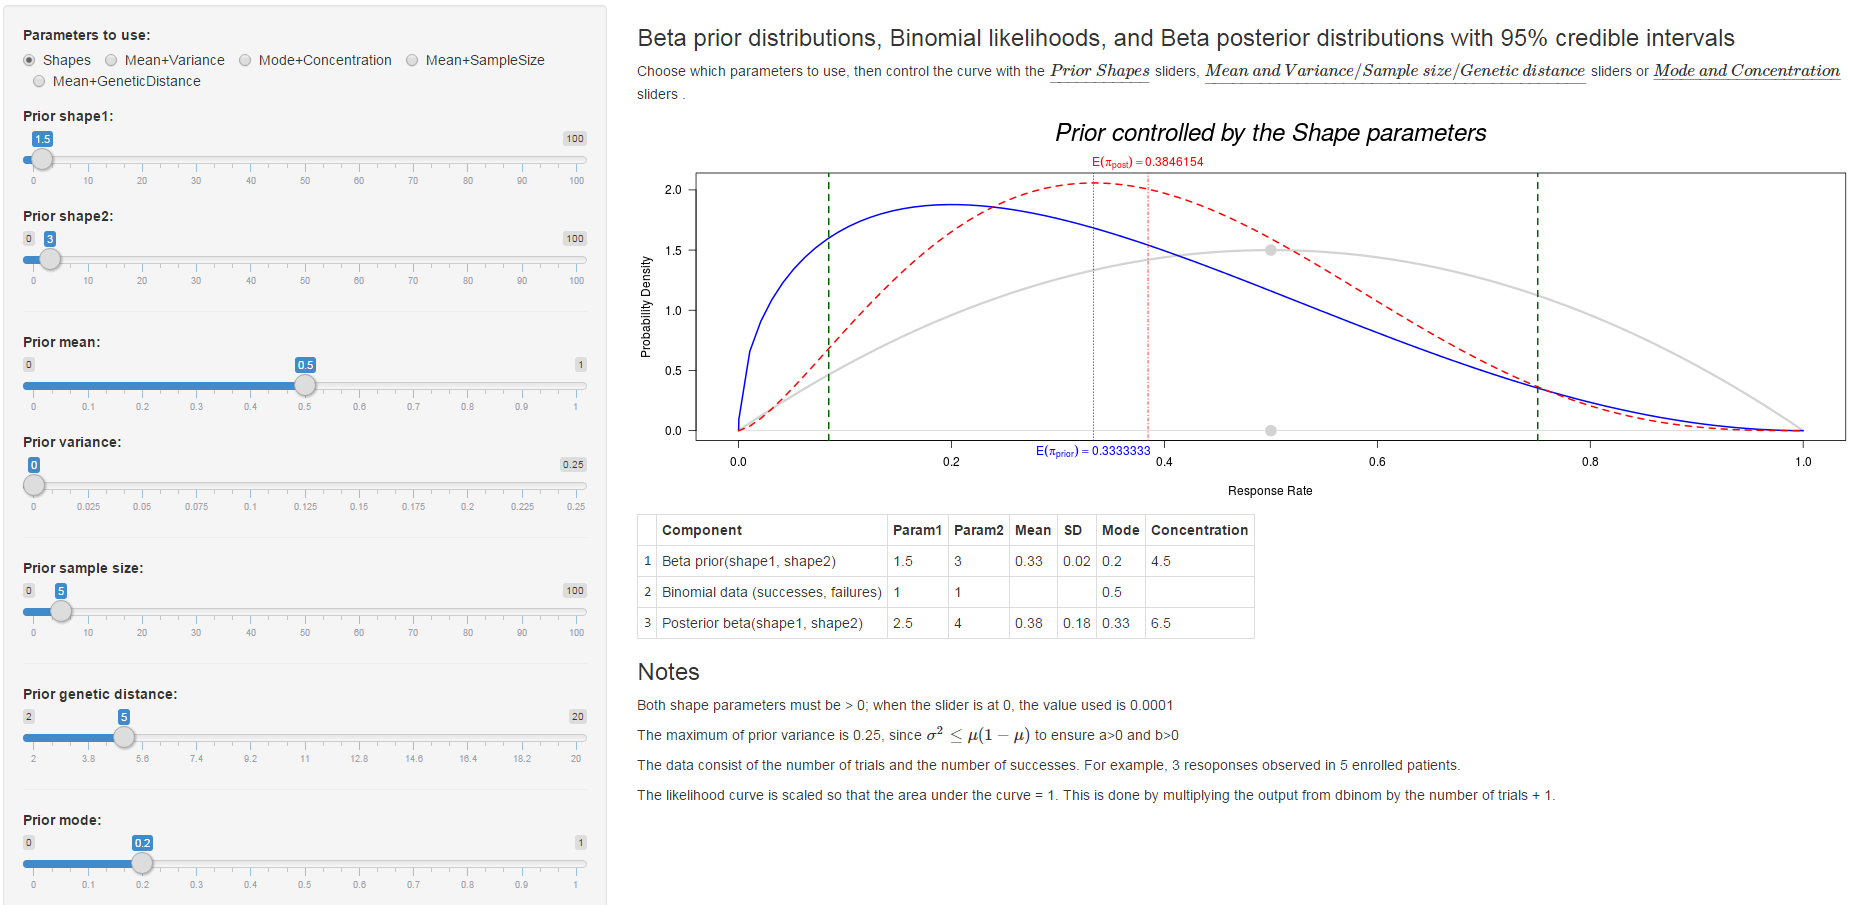
\includegraphics{demo.png}

\end{frame}

\begin{frame}[fragile]{Simulation Example}

Consider \emph{objective response rate} (ORR) as the primary endpoint
with the following hypotheses:
\[H_0: ORR \le 15\% \quad versus \quad H_1: ORR > 15\%.\]

\begin{verbatim}
## Prior: Beta(0.5,0.5)
\end{verbatim}

\animategraphics[width=2.5in,controls,loop]{1}{bayesdesign_files/figure-beamer/unnamed-chunk-6-}{1}{20}

\end{frame}

\begin{frame}[fragile]{Simulation Example (II)}

We can observe after 10 patients enrolled, the difference between
posterior and true response rate reduced to a stable level below 3\%.

\begin{verbatim}
## Prior: Beta(0.5,0.5)
\end{verbatim}

\animategraphics[width=2.5in,controls,loop]{1}{bayesdesign_files/figure-beamer/unnamed-chunk-7-}{1}{10}

\end{frame}

\begin{frame}{Prior selection: Non-informative priors}

\begin{quote}
\begin{enumerate}
\def\labelenumi{\arabic{enumi}.}
\tightlist
\item
  \textbf{Jeffery prior}:

  \begin{itemize}
  \tightlist
  \item
    a=0.5
  \item
    b=0.5
  \end{itemize}
\end{enumerate}

\begin{itemize}
\tightlist
\item
  The prior sample size is 1, mean = 0.5, variance = 0.125 (Data
  dominate)
\item
  \textbf{Remark}: Compared Unif(0,1) prior, whose variance is
  1/12=0.0833, Jeffery prior is more flat and less informative.
\end{itemize}
\end{quote}

\begin{quote}
\begin{enumerate}
\def\labelenumi{\arabic{enumi}.}
\setcounter{enumi}{1}
\tightlist
\item
  \textbf{Optimist's prior}:

  \begin{itemize}
  \tightlist
  \item
    \(a=ORR_{prior}+1\)
  \item
    \(b=(1-ORR_{prior})+1\)
  \end{itemize}
\end{enumerate}

\begin{itemize}
\tightlist
\item
  The prior sample size = 3, centered around \(ORR_{prior}\).
\item
  Such a prior distribution is sufficiently vague to allow for the
  possibility that \(ORR\) may take any value in the range \(0<ORR<1\).
\end{itemize}
\end{quote}

\end{frame}

\begin{frame}{Prior selection: Informative priors:}

\begin{quote}
\begin{enumerate}
\def\labelenumi{\arabic{enumi}.}
\setcounter{enumi}{2}
\tightlist
\item
  \textbf{Based on prior ORR and Sample size (``ORR+N'')}:

  \begin{itemize}
  \tightlist
  \item
    \(a=ORR_{prior}+1+N_{prior}ORR_{prior}\)
  \item
    \(b=(1-ORR_{prior})+1+N_{prior}(1-ORR_{prior})\)
  \end{itemize}
\end{enumerate}

\begin{itemize}
\tightlist
\item
  The prior sample size = \(3+N_{prior}\).
\item
  It is similar to use mean=\(ORR_{prior}\) and variance=
  \(\frac{ORR_{prior}(1-ORR_{prior})}{N_{prior}}\), where the sample
  size = \(N_{prior}-1\)
\end{itemize}
\end{quote}

\begin{quote}
\begin{enumerate}
\def\labelenumi{\arabic{enumi}.}
\setcounter{enumi}{3}
\tightlist
\item
  \textbf{Based on prior ORR and Width of confidence interval
  (``ORR+W'')}:

  \begin{itemize}
  \tightlist
  \item
    \(ORR_{prior}=\dfrac{a}{a+b}\)
  \item
    \(W_{95}=F^{-1}(0.975; a,b)-F^{-1}(0.025; a,b)\)
  \end{itemize}
\end{enumerate}

\begin{itemize}
\tightlist
\item
  Solve the non-linear equations for \(a\) and \(b\)
\end{itemize}
\end{quote}

\end{frame}

\begin{frame}{GO / NO GO Decision: Posterior Probability}

\(PostP=Pr(p>p_0|x)\)

\begin{block}{Algorithm 1}

\begin{itemize}
\tightlist
\item
  \textbf{Step 1:} Specify the upper and lower probability cutoffs
  \(\theta_U\) and \(\theta_L\). Typically, \(\theta_U \in [0.9,1]\) for
  efficacy and \(\theta_L \in [0,0.05]\) for futility, true null
  response rate \(p_0\).
\item
  \textbf{Step 2:} Let
  \[S_U =\min \{x \in \mathbb{N}:  PostP > \theta_U \}\] and
  \[ S_L =\max \{x \in \mathbb{N}:  PostP < \theta_L \}\]
\item
  \textbf{Step 3:} Make decisions after observing another \(x\)
  responses out of \(n\) patients:

  \begin{itemize}
  \tightlist
  \item
    If \(x \ge S_U\), then stop the trial for efficacy;
  \item
    if \(x \le S_L\), then stop the trial for futility;
  \item
    otherwise, continue the trial until \(N_{max}\) reached.
  \end{itemize}
\end{itemize}

\end{block}

\end{frame}

\begin{frame}{GO / NO GO Decision: Predictive Probability}

\(PredP = Pr_{Y|x} \{Pr(p>p_0|x, Y) \ge \theta_T \}\)

\begin{block}{Algorithm 2}

\begin{itemize}
\tightlist
\item
  \textbf{Step 1:} Specified the upper and lower probability cutoffs
  \(\theta_U\) and \(\theta_L\), typically, \(\theta_U \in [0.9,1]\) for
  efficacy and \(\theta_L \in [0,0.05]\) for futility. Specified cutoff
  \(\theta_T\) for the future \(y\) patients, typically,
  \(\theta_T \in [0.8,1]\). Set true null response rate \(p_0\) a
  pre-specified value.
\item
  \textbf{Step 2:} Given \(x\) obwervations, let
  \[S_U =\min \{x+y \in \mathbb{N}:  PredP > \theta_U \}\] and
  \[ S_L =\max \{x+y \in \mathbb{N}:  PredP < \theta_L \}\] be the upper
  and lower decision boudries based on the number of observed responses.
\end{itemize}

\end{block}

\end{frame}

\begin{frame}{GO / NO GO Decision: Predictive Probability}

\(\begin{aligned} PredP & = Pr_{Y|x} \{Pr(p>p_0|x, Y) \ge \theta_T \} \\  & = \sum\limits_{y=0}^{N_{max} -n} I[Pr(p>p_0|x, Y=y) \ge \theta_T] \times Pr(Y=y|x). \label{predp}  \end{aligned}\)

\begin{block}{Algorithm 2 (Cont.)}

\begin{itemize}
\tightlist
\item
  \textbf{Step 3:} Make decisions after observing another \(x\)
  responses out of \(n\) patients:

  \begin{itemize}
  \tightlist
  \item
    If \(x \ge S_U\), then stop the trial for efficacy ;
  \item
    if \(x \le S_L\), then stop the trial for futility;
  \item
    otherwise, continue the trial until \(N_{max}\) reached.
  \end{itemize}
\end{itemize}

\textbf{Remark}: If there were no indicator function in the formula, the
PredP simply reduces to the PostP after averaging out the unobserved Y.

\[\sum\limits_{y=0}^{N_{max} -n}  Pr(p>p_0|x, Y=y) \times Pr(Y=y|x) = Pr(p>p_0|x)\]

\end{block}

\end{frame}

\section{Practical Examples}\label{practical-examples}

\begin{frame}{Design for R2810 Phase II Clinical Trials}

\begin{itemize}[<+->]
\tightlist
\item
  \textbf{Data reference}: R2810 - RECIST (verson 1.1) Overall Response
  Investigator (PD, SD, CR or PR)
\item
  \textbf{Aim of study}: According to current data and prior
  competitors' information, make interim analysis, determine suitable
  stopping rule.
\item
  \textbf{Study design}:

  \begin{itemize}[<+->]
  \tightlist
  \item
    \textbf{Two-stage Design}: Admissible designs
  \item
    \textbf{Sequential monitor}:

    \begin{enumerate}[<+->]
    \def\labelenumi{\arabic{enumi}.}
    \tightlist
    \item
      Posterior probability
    \item
      Predictive probability.
    \end{enumerate}
  \end{itemize}
\item
  \textbf{Outcome measure}: \textbf{ORR} is determined by the proportion
  of patients with best overall response of CR or PR among patients in
  SAF.
\item
  \textbf{Prior information}:

  \begin{enumerate}[<+->]
  \def\labelenumi{\arabic{enumi}.}
  \tightlist
  \item
    \emph{KEYTRUDA} (\(ORR=0.236, N=173, W_{95}=0.186\))
  \item
    \emph{OPDIVO} (\(ORR=0.317, N=120, W_{95}=0.173\))
  \end{enumerate}
\end{itemize}

\end{frame}

\begin{frame}[fragile]{Data Summary}

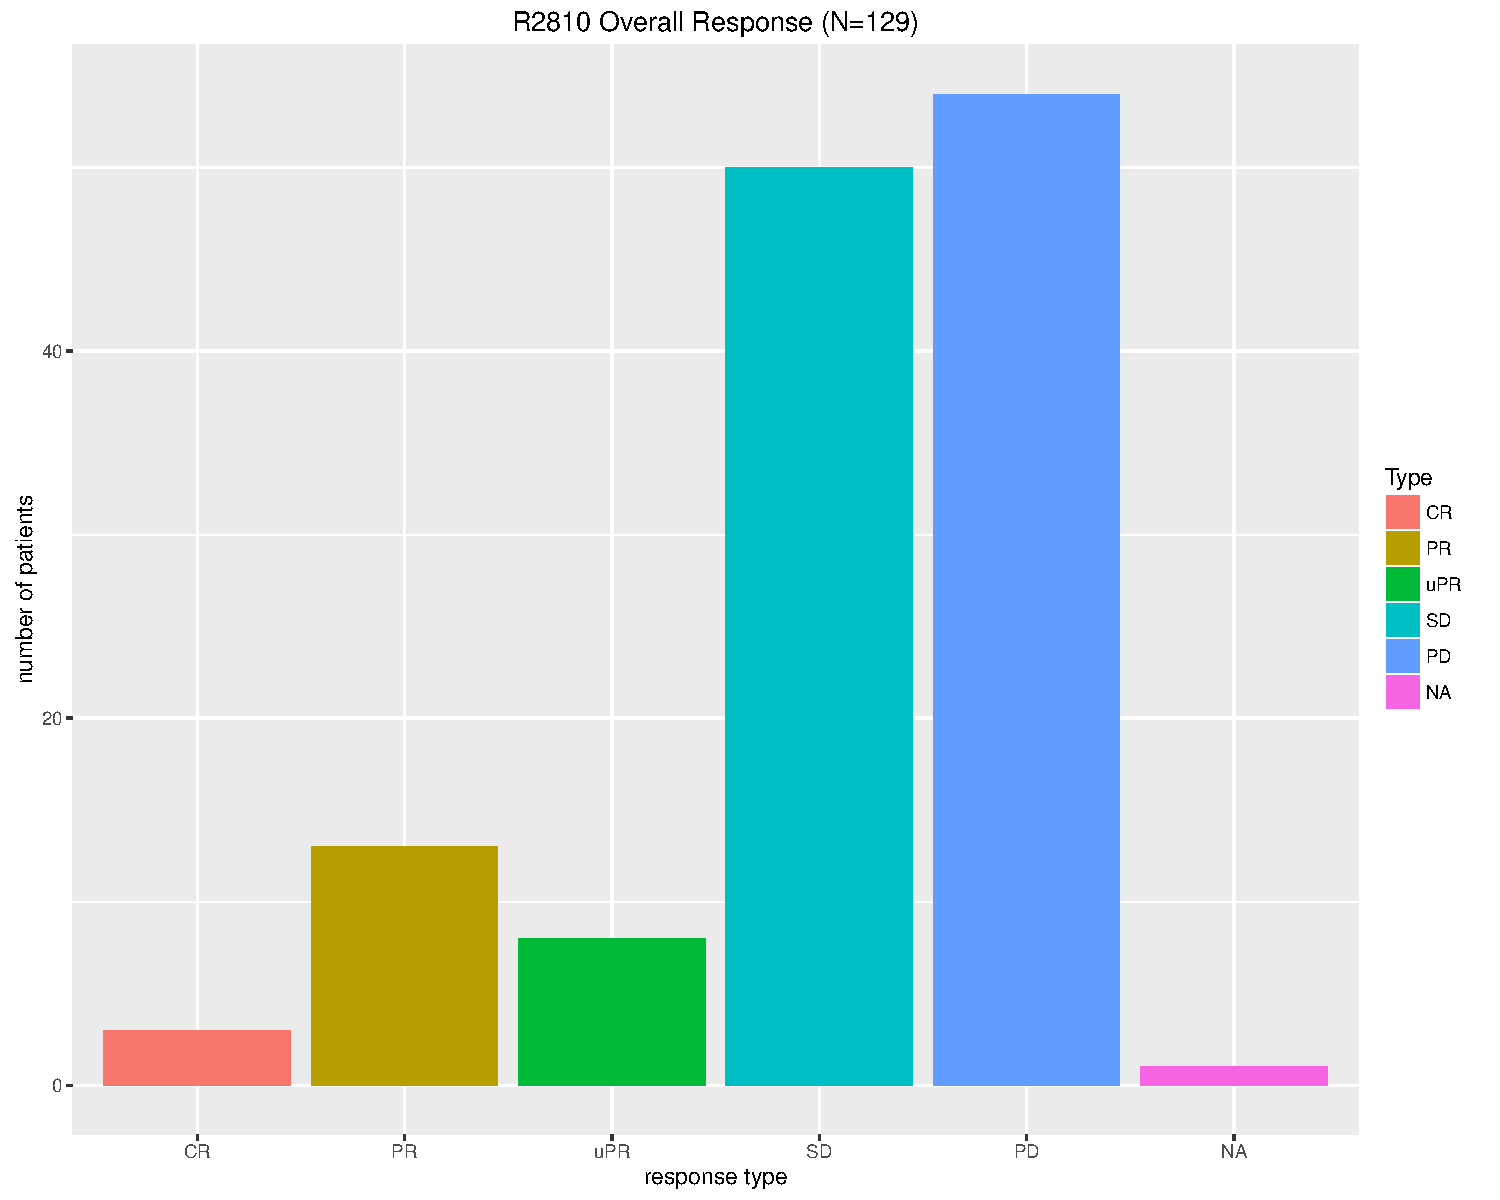
\includegraphics[width=2.46in]{bayesdesign_files/figure-beamer/unnamed-chunk-9-1}
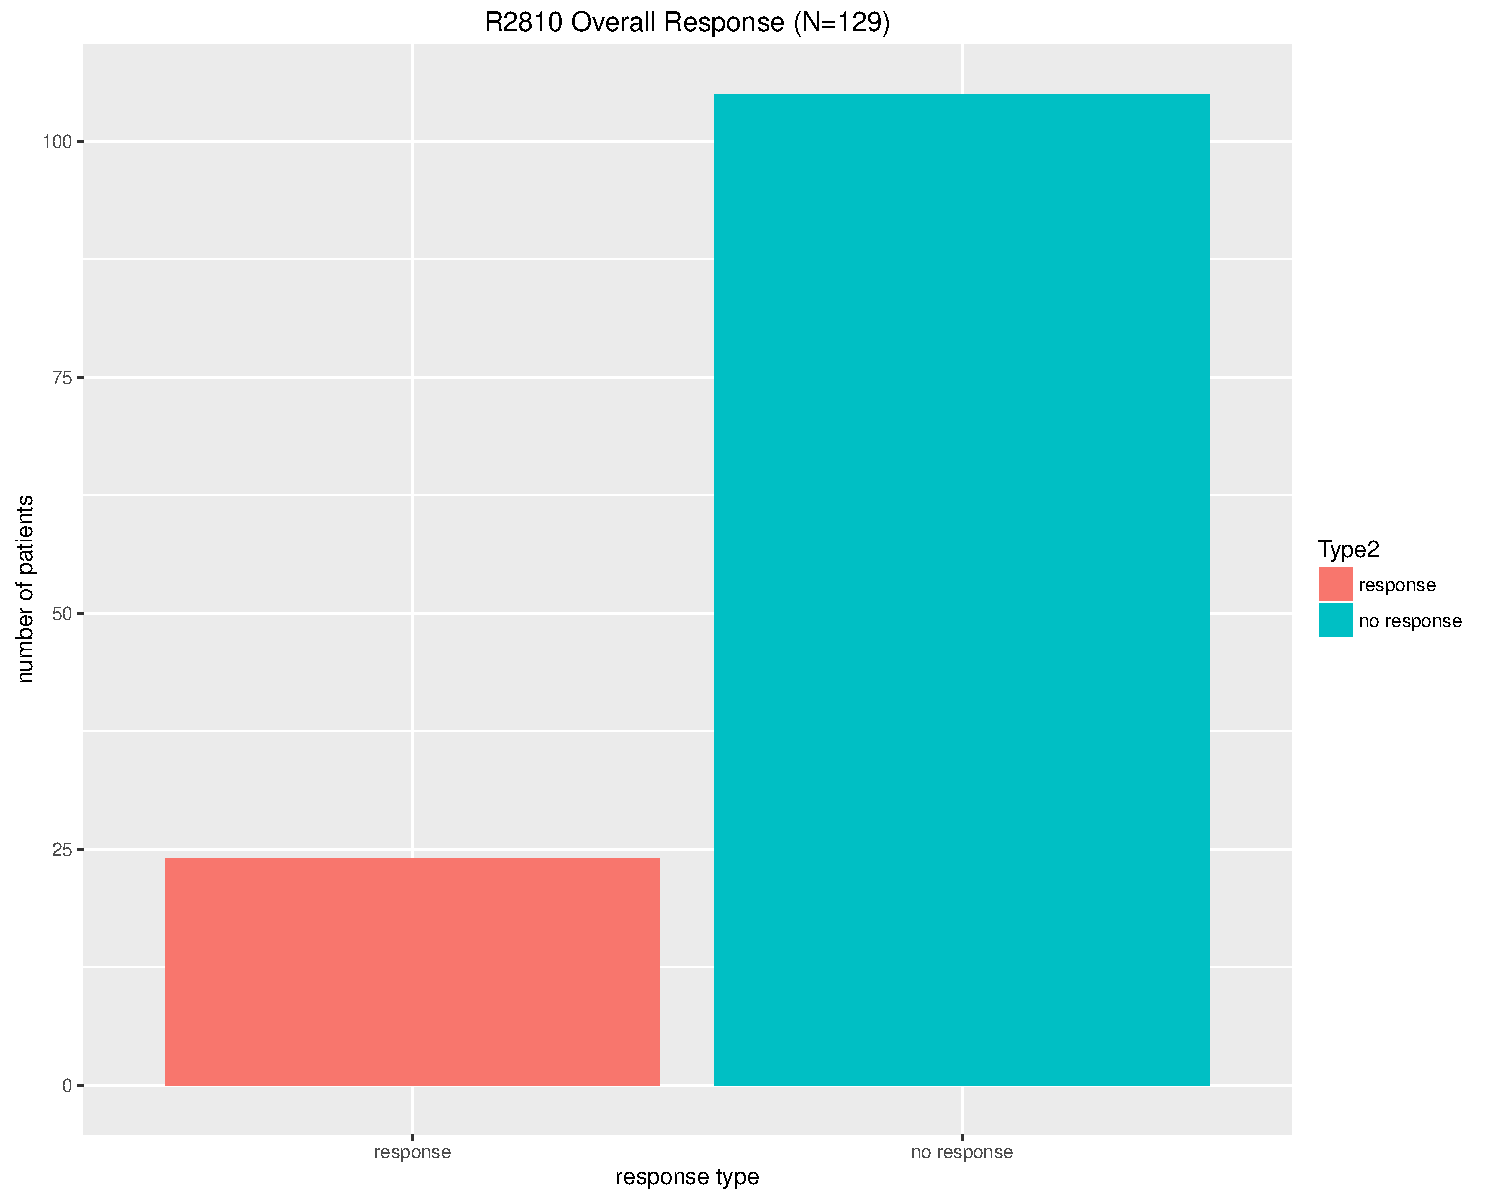
\includegraphics[width=2.46in]{bayesdesign_files/figure-beamer/unnamed-chunk-9-2}

\tiny

\begin{verbatim}
## 
##  Exact binomial test
## 
## data:  sum(r01) and length(r01)
## number of successes = 20, number of trials = 100, p-value = 0.7
## alternative hypothesis: true probability of success is not equal to 0.2
## 95 percent confidence interval:
##  0.123 0.264
## sample estimates:
## probability of success 
##                  0.186
\end{verbatim}

\end{frame}

\begin{frame}{Exact Binomial Test}

Based on the mean \(\mu\) and the variance \(\sigma^2\), we can derive
the prior parameter of \(Beta(a,b)\) distribution with
\[a=\mu\left\{\frac{\mu(1-\mu)}{\sigma^2}-1\right\}\] and
\[b=(1-\mu)\left\{\frac{\mu(1-\mu)}{\sigma^2}-1\right\}.\]

Because of a relationship between the cumulative binomial distribution
and the beta distribution, the Clopper-Pearson interval is sometimes
presented in an alternate format that uses quantiles from the beta
distribution.

\[ B\left(\frac{\alpha}{2}; x, n - x + 1\right) < \theta <  B\left(1 - \frac{\alpha}{2}; x + 1, n - x\right)\]

\end{frame}

\begin{frame}[fragile]{Processing Data By Time-to-event}

\tiny

\begin{Shaded}
\begin{Highlighting}[]
\NormalTok{order.data <-}\StringTok{ }\NormalTok{response[}\KeywordTok{order}\NormalTok{(response$TRTSDTM),}\KeywordTok{c}\NormalTok{(}\StringTok{"TRTSDTM"}\NormalTok{,}\StringTok{"AVALC"}\NormalTok{)]}
\KeywordTok{print}\NormalTok{(}\KeywordTok{cbind}\NormalTok{(}\KeywordTok{head}\NormalTok{(order.data,}\DecValTok{5}\NormalTok{), }\KeywordTok{tail}\NormalTok{(order.data,}\DecValTok{5}\NormalTok{)),}\DataTypeTok{row.names=}\OtherTok{FALSE}\NormalTok{)}
\end{Highlighting}
\end{Shaded}

\begin{verbatim}
##              TRTSDTM AVALC             TRTSDTM AVALC
##  2015-02-04 09:50:00    SD 2016-04-13 11:07:00    SD
##  2015-02-06 09:08:00    PD 2016-04-18 11:05:00    PD
##  2015-02-09 11:15:00    SD 2016-04-18 12:20:00    SD
##  2015-03-16 09:30:00    PD 2016-04-19 08:40:00    PD
##  2015-03-18 09:55:00    PD 2016-04-19 10:42:00    PD
\end{verbatim}

\begin{Shaded}
\begin{Highlighting}[]
\NormalTok{rorder <-}\StringTok{ }\NormalTok{r01[}\KeywordTok{order}\NormalTok{(response$TRTSDTM)]}
\NormalTok{rorder}
\end{Highlighting}
\end{Shaded}

\begin{verbatim}
##   [1] 0 0 0 0 0 0 0 1 1 0 0 0 0 0 0 0 0 0 1 0 0 0 0 0 0 0 0 1 1 0 0 1 0 1 0
##  [36] 0 0 1 1 0 0 1 0 0 1 1 0 0 0 1 0 0 0 0 0 0 1 0 0 0 0 0 0 0 0 0 0 0 0 0
##  [71] 0 0 1 0 0 0 0 0 0 0 0 0 0 0 0 1 0 0 0 0 1 0 1 0 0 0 0 0 0 0 0 0 0 0 0
## [106] 0 1 0 0 1 1 0 0 1 0 0 0 1 0 0 1 0 0 0 0 0 0 0 0
\end{verbatim}

\begin{Shaded}
\begin{Highlighting}[]
\NormalTok{rtotal <-}\StringTok{ }\KeywordTok{cumsum}\NormalTok{(r01[}\KeywordTok{order}\NormalTok{(response$TRTSDTM)])}
\NormalTok{rtotal}
\end{Highlighting}
\end{Shaded}

\begin{verbatim}
##   [1]  0  0  0  0  0  0  0  1  2  2  2  2  2  2  2  2  2  2  3  3  3  3  3
##  [24]  3  3  3  3  4  5  5  5  6  6  7  7  7  7  8  9  9  9 10 10 10 11 12
##  [47] 12 12 12 13 13 13 13 13 13 13 14 14 14 14 14 14 14 14 14 14 14 14 14
##  [70] 14 14 14 15 15 15 15 15 15 15 15 15 15 15 15 15 16 16 16 16 16 17 17
##  [93] 18 18 18 18 18 18 18 18 18 18 18 18 18 18 19 19 19 20 21 21 21 22 22
## [116] 22 22 23 23 23 24 24 24 24 24 24 24 24 24
\end{verbatim}

\end{frame}

\begin{frame}[fragile]{Two-stage Design Analysis}

We can use the following program to run the two-stage designs (Optimal,
Minimax and Admissible) \tiny

\begin{Shaded}
\begin{Highlighting}[]
\KeywordTok{binom.design}\NormalTok{(}\DataTypeTok{output=}\StringTok{"admissible"}\NormalTok{, }\DataTypeTok{p0=}\FloatTok{0.1}\NormalTok{, }\DataTypeTok{p1=}\FloatTok{0.3}\NormalTok{, }\DataTypeTok{signif.level =} \FloatTok{0.05}\NormalTok{, }\DataTypeTok{power.level =} \FloatTok{0.9}\NormalTok{)}
\end{Highlighting}
\end{Shaded}

\begin{verbatim}
##            r1 n1 r  n EN.p0. PET.p0.  error power
## Optimal     2 18 6 35   22.5   0.734 0.0474 0.902
## Admissible  2 19 6 34   23.4   0.705 0.0438 0.901
## Minimax     2 22 6 33   26.2   0.620 0.0409 0.902
\end{verbatim}

\begin{table}[ht]  \fontsize{7}{9}\selectfont
\centering
\begin{tabular}{crrrrrrrrr}
  \hline
 & & r1(data) & n1 & r(data) & n & EN.p0. & PET.p0. & error & power \\ 
  \hline
Scenario 1 &  Optimal & 2(2) & 18 & 6(7) & 35 & 22.5255 & 0.7338 & 0.0474 & 0.9016 \\ 
$p_0=0.1$ & Admissible & 2(3) & 19 & 6(7) & 34 & 23.4183 & 0.7054 & 0.0438 & 0.9014 \\ 
$p_1=0.3$ & Minimax & 2(3) & 22 & 6(6) & 33 & 26.1795 & 0.6200 & 0.0409 & 0.9018 \\ 
   \hline
Scenario 2 & Optimal & 4(3) & 19 & 15(13) & 54 & 30.4349 & 0.6733 & 0.0482 & 0.9045 \\ 
$p_0=0.2$ &  Admissible & 4(3) & 20 & 14(12) & 49 & 30.7402 & 0.6296 & 0.0457 & 0.9030 \\ 
$p_1=0.4$ &  Minimax & 5(3) & 24 & 13(11) & 45 & 31.2263 & 0.6559 & 0.0483 & 0.9001 \\ 
   \hline  
Scenario 3 &   Optimal & 13(3) & 24 & 36(14) & 61 & 34.0132 & 0.7294 & 0.0487 & 0.9014 \\ 
$p_0=0.5$ &  Admissible & 12(3) & 23 & 34(14) & 57 & 34.5199 & 0.6612 & 0.0482 & 0.9046 \\ 
$p_1=0.7$ &  Minimax & 14(3) & 27 & 32(13) & 53 & 36.1144 & 0.6494 & 0.0461 & 0.9004 \\ 
   \hline
\end{tabular}
\tiny{\caption{Illustration of Simon's two-stage designs with three scenarios of design parameters, under the constraints on $\alpha=0.05$ and $1-\beta=0.9$.}} 
\end{table}

\end{frame}

\begin{frame}{Results for two-stage designs}

Except the \textbf{admissible} and \textbf{minimax} design under
\textbf{Scenario 1 (\(p_0=0.1\), \(p_1=0.3\))}, other designs will be
early terminated for futility for our data.

\textbf{We have not used any prior information, although we have!}


\includegraphics{dwyl.jpg}

\end{frame}

\begin{frame}[fragile]{Seqential Monitor: \texttt{PostP\ Design}}

The Bayesian designs provide a seqence of stopping boundary for response
with corresponding sample size. Theoretically we can sequentially
monitor the trial based on these rules.

Programming Examples: \textbf{Jeffery prior} \(a=b=0.5\)

\tiny

\begin{Shaded}
\begin{Highlighting}[]
\KeywordTok{library}\NormalTok{(dplyr)}
\KeywordTok{library}\NormalTok{(ph2bye)}
\KeywordTok{PostP.design}\NormalTok{(}\DataTypeTok{type =} \StringTok{"futility"}\NormalTok{, }\DataTypeTok{nmax =} \DecValTok{129}\NormalTok{, }\DataTypeTok{a=}\FloatTok{0.5}\NormalTok{, }\DataTypeTok{b=}\FloatTok{0.5}\NormalTok{, }\DataTypeTok{p0=}\FloatTok{0.4}\NormalTok{, }\DataTypeTok{theta =} \FloatTok{0.05}\NormalTok{) %>%}\StringTok{ }\KeywordTok{filter}\NormalTok{(bound %in%}\StringTok{ }\KeywordTok{c}\NormalTok{(}\DecValTok{4}\NormalTok{,}\DecValTok{5}\NormalTok{,}\DecValTok{13}\NormalTok{,}\DecValTok{14}\NormalTok{,}\DecValTok{15}\NormalTok{)) }\CommentTok{# filter the design based on Simon's minimum sample size for first stage}
\end{Highlighting}
\end{Shaded}

\begin{verbatim}
##    n bound
## 1 19     4
## 2 22     5
## 3 46    13
## 4 49    14
## 5 52    15
\end{verbatim}

\begin{Shaded}
\begin{Highlighting}[]
\KeywordTok{simon.power}\NormalTok{(}\DataTypeTok{r1 =} \DecValTok{4}\NormalTok{, }\DataTypeTok{n1=}\DecValTok{19}\NormalTok{, }\DataTypeTok{r=}\DecValTok{15}\NormalTok{, }\DataTypeTok{n=}\DecValTok{52}\NormalTok{, }\DataTypeTok{p =} \FloatTok{0.2}\NormalTok{) }
\end{Highlighting}
\end{Shaded}

\begin{verbatim}
## [1] 0.0366
\end{verbatim}

\begin{Shaded}
\begin{Highlighting}[]
\KeywordTok{PostP.design}\NormalTok{(}\DataTypeTok{type =} \StringTok{"efficacy"}\NormalTok{, }\DataTypeTok{nmax =} \DecValTok{129}\NormalTok{, }\DataTypeTok{a=}\FloatTok{0.5}\NormalTok{, }\DataTypeTok{b=}\FloatTok{0.5}\NormalTok{, }\DataTypeTok{p0=}\FloatTok{0.2}\NormalTok{, }\DataTypeTok{theta =} \FloatTok{0.9}\NormalTok{)%>%}\StringTok{ }\KeywordTok{filter}\NormalTok{(bound %in%}\StringTok{ }\KeywordTok{c}\NormalTok{(}\DecValTok{4}\NormalTok{,}\DecValTok{5}\NormalTok{,}\DecValTok{13}\NormalTok{,}\DecValTok{14}\NormalTok{,}\DecValTok{15}\NormalTok{))}
\end{Highlighting}
\end{Shaded}

\begin{verbatim}
##    n bound
## 1  8     4
## 2 12     5
## 3 43    13
## 4 48    14
## 5 52    15
\end{verbatim}

\begin{Shaded}
\begin{Highlighting}[]
\KeywordTok{simon.power}\NormalTok{(}\DataTypeTok{r1 =} \DecValTok{4}\NormalTok{, }\DataTypeTok{n1=}\DecValTok{9}\NormalTok{, }\DataTypeTok{r=}\DecValTok{15}\NormalTok{, }\DataTypeTok{n=}\DecValTok{53}\NormalTok{, }\DataTypeTok{p =} \FloatTok{0.4}\NormalTok{) }
\end{Highlighting}
\end{Shaded}

\begin{verbatim}
## [1] 0.264
\end{verbatim}

\begin{Shaded}
\begin{Highlighting}[]
\KeywordTok{ani.options}\NormalTok{(}\DataTypeTok{convert=}\StringTok{'C:}\CharTok{\textbackslash{}\textbackslash{}}\StringTok{Users}\CharTok{\textbackslash{}\textbackslash{}}\StringTok{yalin.zhu}\CharTok{\textbackslash{}\textbackslash{}}\StringTok{Documents}\CharTok{\textbackslash{}\textbackslash{}}\StringTok{ImageMagick-7.0.1-10-portable-Q16-x64}\CharTok{\textbackslash{}\textbackslash{}}\StringTok{convert.exe'}\NormalTok{)}

\KeywordTok{BB.aniplot}\NormalTok{(}\DataTypeTok{a =} \FloatTok{0.5}\NormalTok{, }\DataTypeTok{b =} \FloatTok{0.5}\NormalTok{, }\DataTypeTok{r =} \NormalTok{r01, }\DataTypeTok{N =} \DecValTok{1}\NormalTok{, }\DataTypeTok{time.interval =} \FloatTok{0.01}\NormalTok{, }\DataTypeTok{output =} \NormalTok{F)}

\KeywordTok{bayes.design}\NormalTok{(}\DataTypeTok{a =} \FloatTok{0.5}\NormalTok{, }\DataTypeTok{b =} \FloatTok{0.5}\NormalTok{, }\DataTypeTok{r =} \NormalTok{rorder, }\DataTypeTok{stop.rule =} \StringTok{"futility"}\NormalTok{, }\DataTypeTok{p0 =} \FloatTok{0.4}\NormalTok{, }\DataTypeTok{time.interval =} \FloatTok{0.1}\NormalTok{)}
\KeywordTok{bayes.design}\NormalTok{(}\DataTypeTok{a =} \FloatTok{0.5}\NormalTok{, }\DataTypeTok{b =} \FloatTok{0.5}\NormalTok{, }\DataTypeTok{r =} \NormalTok{rorder, }\DataTypeTok{stop.rule =} \StringTok{"efficacy"}\NormalTok{, }\DataTypeTok{p0 =} \FloatTok{0.2}\NormalTok{, }\DataTypeTok{time.interval =} \FloatTok{0.1}\NormalTok{)}
\end{Highlighting}
\end{Shaded}

\begin{Shaded}
\begin{Highlighting}[]
\KeywordTok{source}\NormalTok{(}\StringTok{"prior_fun.R"}\NormalTok{)}
\end{Highlighting}
\end{Shaded}

\end{frame}

\begin{frame}[fragile]{Optimist's prior: KEYTRUDA : \(a=1.24, b=1.76\)}

\tiny

\begin{Shaded}
\begin{Highlighting}[]
\NormalTok{KT.prior <-}\StringTok{ }\KeywordTok{optprior}\NormalTok{(KT.mean); KT.prior }\CommentTok{# KEYTRUDA optimist's prior}
\end{Highlighting}
\end{Shaded}

\begin{verbatim}
##    a    b 
## 1.24 1.76
\end{verbatim}

\begin{Shaded}
\begin{Highlighting}[]
\KeywordTok{PostP.design}\NormalTok{(}\DataTypeTok{type =} \StringTok{"futility"}\NormalTok{, }\DataTypeTok{nmax =} \DecValTok{129}\NormalTok{, }\DataTypeTok{a=}\FloatTok{1.24}\NormalTok{, }\DataTypeTok{b=}\FloatTok{1.76}\NormalTok{, }\DataTypeTok{p0=}\FloatTok{0.4}\NormalTok{, }\DataTypeTok{theta =} \FloatTok{0.05}\NormalTok{) %>%}\StringTok{ }\KeywordTok{filter}\NormalTok{(bound %in%}\StringTok{ }\KeywordTok{c}\NormalTok{(}\DecValTok{4}\NormalTok{,}\DecValTok{5}\NormalTok{,}\DecValTok{13}\NormalTok{,}\DecValTok{14}\NormalTok{,}\DecValTok{15}\NormalTok{)) }\CommentTok{# filter the design based on Simon's minimum sample size for first stage}
\end{Highlighting}
\end{Shaded}

\begin{verbatim}
##    n bound
## 1 19     4
## 2 23     5
## 3 47    13
## 4 50    14
## 5 52    15
\end{verbatim}

\begin{Shaded}
\begin{Highlighting}[]
\KeywordTok{PostP.design}\NormalTok{(}\DataTypeTok{type =} \StringTok{"efficacy"}\NormalTok{, }\DataTypeTok{nmax =} \DecValTok{129}\NormalTok{, }\DataTypeTok{a=}\FloatTok{1.24}\NormalTok{, }\DataTypeTok{b=}\FloatTok{1.76}\NormalTok{, }\DataTypeTok{p0=}\FloatTok{0.2}\NormalTok{, }\DataTypeTok{theta =} \FloatTok{0.9}\NormalTok{)%>%}\StringTok{ }\KeywordTok{filter}\NormalTok{(bound %in%}\StringTok{ }\KeywordTok{c}\NormalTok{(}\DecValTok{4}\NormalTok{,}\DecValTok{5}\NormalTok{,}\DecValTok{13}\NormalTok{,}\DecValTok{14}\NormalTok{,}\DecValTok{15}\NormalTok{))}
\end{Highlighting}
\end{Shaded}

\begin{verbatim}
##    n bound
## 1  9     4
## 2 12     5
## 3 45    13
## 4 49    14
## 5 53    15
\end{verbatim}

\begin{Shaded}
\begin{Highlighting}[]
\KeywordTok{bayes.design}\NormalTok{(}\DataTypeTok{a =} \FloatTok{1.24}\NormalTok{, }\DataTypeTok{b =} \FloatTok{1.76}\NormalTok{, }\DataTypeTok{r =} \NormalTok{rorder, }\DataTypeTok{stop.rule =} \StringTok{"futility"}\NormalTok{, }\DataTypeTok{p0 =} \FloatTok{0.4}\NormalTok{, }\DataTypeTok{time.interval =} \FloatTok{0.1}\NormalTok{)}
\KeywordTok{bayes.design}\NormalTok{(}\DataTypeTok{a =} \FloatTok{1.24}\NormalTok{, }\DataTypeTok{b =} \FloatTok{1.76}\NormalTok{, }\DataTypeTok{r =} \NormalTok{rorder, }\DataTypeTok{stop.rule =} \StringTok{"efficacy"}\NormalTok{, }\DataTypeTok{p0 =} \FloatTok{0.2}\NormalTok{, }\DataTypeTok{time.interval =} \FloatTok{0.1}\NormalTok{)}
\end{Highlighting}
\end{Shaded}

\end{frame}

\begin{frame}[fragile]{Optimist's prior: OPDIVO : \(a=1.32, b=1.68\)}

\tiny

\begin{Shaded}
\begin{Highlighting}[]
\NormalTok{OD.prior <-}\StringTok{ }\KeywordTok{optprior}\NormalTok{(OD.mean); OD.prior }\CommentTok{# OPDIVO optimist's prior}
\end{Highlighting}
\end{Shaded}

\begin{verbatim}
##    a    b 
## 1.32 1.68
\end{verbatim}

\begin{Shaded}
\begin{Highlighting}[]
\KeywordTok{PostP.design}\NormalTok{(}\DataTypeTok{type =} \StringTok{"futility"}\NormalTok{, }\DataTypeTok{nmax =} \DecValTok{129}\NormalTok{, }\DataTypeTok{a=}\FloatTok{1.32}\NormalTok{, }\DataTypeTok{b=}\FloatTok{1.68}\NormalTok{, }\DataTypeTok{p0=}\FloatTok{0.4}\NormalTok{, }\DataTypeTok{theta =} \FloatTok{0.05}\NormalTok{) %>%}\StringTok{ }\KeywordTok{filter}\NormalTok{(bound %in%}\StringTok{ }\KeywordTok{c}\NormalTok{(}\DecValTok{4}\NormalTok{,}\DecValTok{5}\NormalTok{,}\DecValTok{13}\NormalTok{,}\DecValTok{14}\NormalTok{,}\DecValTok{15}\NormalTok{)) }\CommentTok{# filter the design based on Simon's minimum sample size for first stage}
\end{Highlighting}
\end{Shaded}

\begin{verbatim}
##    n bound
## 1 20     4
## 2 23     5
## 3 47    13
## 4 50    14
## 5 53    15
\end{verbatim}

\begin{Shaded}
\begin{Highlighting}[]
\KeywordTok{PostP.design}\NormalTok{(}\DataTypeTok{type =} \StringTok{"efficacy"}\NormalTok{, }\DataTypeTok{nmax =} \DecValTok{129}\NormalTok{, }\DataTypeTok{a=}\FloatTok{1.32}\NormalTok{, }\DataTypeTok{b=}\FloatTok{1.68}\NormalTok{, }\DataTypeTok{p0=}\FloatTok{0.2}\NormalTok{, }\DataTypeTok{theta =} \FloatTok{0.9}\NormalTok{)%>%}\StringTok{ }\KeywordTok{filter}\NormalTok{(bound %in%}\StringTok{ }\KeywordTok{c}\NormalTok{(}\DecValTok{4}\NormalTok{,}\DecValTok{5}\NormalTok{,}\DecValTok{13}\NormalTok{,}\DecValTok{14}\NormalTok{,}\DecValTok{15}\NormalTok{))}
\end{Highlighting}
\end{Shaded}

\begin{verbatim}
##    n bound
## 1  9     4
## 2 13     5
## 3 45    13
## 4 49    14
## 5 53    15
\end{verbatim}

\begin{Shaded}
\begin{Highlighting}[]
\KeywordTok{bayes.design}\NormalTok{(}\DataTypeTok{a=}\FloatTok{1.32}\NormalTok{, }\DataTypeTok{b=}\FloatTok{1.68}\NormalTok{, }\DataTypeTok{r =} \NormalTok{rorder, }\DataTypeTok{stop.rule =} \StringTok{"futility"}\NormalTok{, }\DataTypeTok{p0 =} \FloatTok{0.4}\NormalTok{, }\DataTypeTok{time.interval =} \FloatTok{0.1}\NormalTok{)}
\KeywordTok{bayes.design}\NormalTok{(}\DataTypeTok{a=}\FloatTok{1.32}\NormalTok{, }\DataTypeTok{b=}\FloatTok{1.68}\NormalTok{, }\DataTypeTok{r =} \NormalTok{rorder, }\DataTypeTok{stop.rule =} \StringTok{"efficacy"}\NormalTok{, }\DataTypeTok{p0 =} \FloatTok{0.2}\NormalTok{, }\DataTypeTok{time.interval =} \FloatTok{0.1}\NormalTok{)}
\end{Highlighting}
\end{Shaded}

\end{frame}

\begin{frame}[fragile]{ORR+N prior: KEYTRUDA : \(a=42.1, b=133.9\)}

\tiny

\begin{Shaded}
\begin{Highlighting}[]
\NormalTok{KT.prior <-}\StringTok{ }\KeywordTok{ORRNprior}\NormalTok{(KT.mean, KT.n); KT.prior }\CommentTok{# KEYTRUDA optimist's prior}
\end{Highlighting}
\end{Shaded}

\begin{verbatim}
##     a     b 
##  42.1 133.9
\end{verbatim}

\begin{Shaded}
\begin{Highlighting}[]
\KeywordTok{PostP.design}\NormalTok{(}\DataTypeTok{type =} \StringTok{"futility"}\NormalTok{, }\DataTypeTok{nmax =} \DecValTok{129}\NormalTok{, }\DataTypeTok{a=}\FloatTok{42.1}\NormalTok{, }\DataTypeTok{b=}\FloatTok{133.9}\NormalTok{, }\DataTypeTok{p0=}\FloatTok{0.4}\NormalTok{, }\DataTypeTok{theta =} \FloatTok{0.05}\NormalTok{) %>%}\StringTok{ }\KeywordTok{filter}\NormalTok{(bound %in%}\StringTok{ }\KeywordTok{c}\NormalTok{(}\DecValTok{4}\NormalTok{,}\DecValTok{5}\NormalTok{,}\DecValTok{13}\NormalTok{,}\DecValTok{14}\NormalTok{,}\DecValTok{15}\NormalTok{)) }\CommentTok{# filter the design based on Simon's minimum sample size for first stage}
\end{Highlighting}
\end{Shaded}

\begin{verbatim}
##    n bound
## 1  4     4
## 2  5     5
## 3 13    13
## 4 14    14
## 5 15    15
\end{verbatim}

\begin{Shaded}
\begin{Highlighting}[]
\KeywordTok{PostP.design}\NormalTok{(}\DataTypeTok{type =} \StringTok{"efficacy"}\NormalTok{, }\DataTypeTok{nmax =} \DecValTok{129}\NormalTok{, }\DataTypeTok{a=}\FloatTok{42.1}\NormalTok{, }\DataTypeTok{b=}\FloatTok{133.9}\NormalTok{, }\DataTypeTok{p0=}\FloatTok{0.2}\NormalTok{, }\DataTypeTok{theta =} \FloatTok{0.9}\NormalTok{)%>%}\StringTok{ }\KeywordTok{filter}\NormalTok{(bound %in%}\StringTok{ }\KeywordTok{c}\NormalTok{(}\DecValTok{4}\NormalTok{,}\DecValTok{5}\NormalTok{,}\DecValTok{13}\NormalTok{,}\DecValTok{14}\NormalTok{,}\DecValTok{15}\NormalTok{))}
\end{Highlighting}
\end{Shaded}

\begin{verbatim}
##    n bound
## 1 13     4
## 2 18     5
## 3 54    13
## 4 59    14
## 5 64    15
\end{verbatim}

\begin{Shaded}
\begin{Highlighting}[]
\KeywordTok{bayes.design}\NormalTok{(}\DataTypeTok{a=}\FloatTok{42.1}\NormalTok{, }\DataTypeTok{b=}\FloatTok{133.9}\NormalTok{, }\DataTypeTok{r =} \NormalTok{rorder, }\DataTypeTok{stop.rule =} \StringTok{"futility"}\NormalTok{, }\DataTypeTok{p0 =} \FloatTok{0.4}\NormalTok{, }\DataTypeTok{time.interval =} \FloatTok{0.1}\NormalTok{)}
\KeywordTok{bayes.design}\NormalTok{(}\DataTypeTok{a=}\FloatTok{42.1}\NormalTok{, }\DataTypeTok{b=}\FloatTok{133.9}\NormalTok{, }\DataTypeTok{r =} \NormalTok{rorder, }\DataTypeTok{stop.rule =} \StringTok{"efficacy"}\NormalTok{, }\DataTypeTok{p0 =} \FloatTok{0.2}\NormalTok{, }\DataTypeTok{time.interval =} \FloatTok{0.1}\NormalTok{)}
\end{Highlighting}
\end{Shaded}

\end{frame}

\begin{frame}[fragile]{ORR+N prior: KEYTRUDA : \(a=39.4, b=83.6\)}

\tiny

\begin{Shaded}
\begin{Highlighting}[]
\NormalTok{OD.prior <-}\StringTok{ }\KeywordTok{ORRNprior}\NormalTok{(OD.mean, OD.n); OD.prior }\CommentTok{# OPDIVO optimist's prior}
\end{Highlighting}
\end{Shaded}

\begin{verbatim}
##    a    b 
## 39.4 83.6
\end{verbatim}

\begin{Shaded}
\begin{Highlighting}[]
\KeywordTok{PostP.design}\NormalTok{(}\DataTypeTok{type =} \StringTok{"futility"}\NormalTok{, }\DataTypeTok{nmax =} \DecValTok{129}\NormalTok{, }\DataTypeTok{a=}\FloatTok{39.4}\NormalTok{, }\DataTypeTok{b=}\FloatTok{83.6}\NormalTok{, }\DataTypeTok{p0=}\FloatTok{0.4}\NormalTok{, }\DataTypeTok{theta =} \FloatTok{0.05}\NormalTok{) %>%}\StringTok{ }\KeywordTok{filter}\NormalTok{(bound %in%}\StringTok{ }\KeywordTok{c}\NormalTok{(}\DecValTok{4}\NormalTok{,}\DecValTok{5}\NormalTok{,}\DecValTok{13}\NormalTok{,}\DecValTok{14}\NormalTok{,}\DecValTok{15}\NormalTok{)) }\CommentTok{# filter the design based on Simon's minimum sample size for first stage}
\end{Highlighting}
\end{Shaded}

\begin{verbatim}
##    n bound
## 1  9     4
## 2 11     5
## 3 33    13
## 4 36    14
## 5 39    15
\end{verbatim}

\begin{Shaded}
\begin{Highlighting}[]
\KeywordTok{PostP.design}\NormalTok{(}\DataTypeTok{type =} \StringTok{"efficacy"}\NormalTok{, }\DataTypeTok{nmax =} \DecValTok{129}\NormalTok{, }\DataTypeTok{a=}\FloatTok{39.4}\NormalTok{, }\DataTypeTok{b=}\FloatTok{83.6}\NormalTok{, }\DataTypeTok{p0=}\FloatTok{0.2}\NormalTok{, }\DataTypeTok{theta =} \FloatTok{0.9}\NormalTok{)%>%}\StringTok{ }\KeywordTok{filter}\NormalTok{(bound %in%}\StringTok{ }\KeywordTok{c}\NormalTok{(}\DecValTok{4}\NormalTok{,}\DecValTok{5}\NormalTok{,}\DecValTok{13}\NormalTok{,}\DecValTok{14}\NormalTok{,}\DecValTok{15}\NormalTok{))}
\end{Highlighting}
\end{Shaded}

\begin{verbatim}
##     n bound
## 1  54     4
## 2  58     5
## 3  95    13
## 4 100    14
## 5 104    15
\end{verbatim}

\begin{Shaded}
\begin{Highlighting}[]
\KeywordTok{bayes.design}\NormalTok{(}\DataTypeTok{a=}\FloatTok{39.4}\NormalTok{, }\DataTypeTok{b=}\FloatTok{83.6}\NormalTok{, }\DataTypeTok{r =} \NormalTok{rorder, }\DataTypeTok{stop.rule =} \StringTok{"futility"}\NormalTok{, }\DataTypeTok{p0 =} \FloatTok{0.4}\NormalTok{, }\DataTypeTok{time.interval =} \FloatTok{0.1}\NormalTok{)}
\KeywordTok{bayes.design}\NormalTok{(}\DataTypeTok{a=}\FloatTok{39.4}\NormalTok{, }\DataTypeTok{b=}\FloatTok{83.6}\NormalTok{, }\DataTypeTok{r =} \NormalTok{rorder, }\DataTypeTok{stop.rule =} \StringTok{"efficacy"}\NormalTok{, }\DataTypeTok{p0 =} \FloatTok{0.2}\NormalTok{, }\DataTypeTok{time.interval =} \FloatTok{0.1}\NormalTok{)}
\end{Highlighting}
\end{Shaded}

\end{frame}

\begin{frame}[fragile]{ORR+W prior: KEYTRUDA: \(a=18.5, b=59.9\)}

\tiny

\begin{Shaded}
\begin{Highlighting}[]
\NormalTok{KT.prior <-}\StringTok{ }\KeywordTok{ORRWprior}\NormalTok{(KT.mean, KT.W);  }\CommentTok{# KEYTRUDA optimist's prior}
\end{Highlighting}
\end{Shaded}

\tiny

\begin{Shaded}
\begin{Highlighting}[]
\KeywordTok{PostP.design}\NormalTok{(}\DataTypeTok{type =} \StringTok{"futility"}\NormalTok{, }\DataTypeTok{nmax =} \DecValTok{129}\NormalTok{, }\DataTypeTok{a=}\FloatTok{18.5}\NormalTok{, }\DataTypeTok{b=}\FloatTok{59.9}\NormalTok{, }\DataTypeTok{p0=}\FloatTok{0.4}\NormalTok{, }\DataTypeTok{theta =} \FloatTok{0.05}\NormalTok{) %>%}\StringTok{ }\KeywordTok{filter}\NormalTok{(bound %in%}\StringTok{ }\KeywordTok{c}\NormalTok{(}\DecValTok{4}\NormalTok{,}\DecValTok{5}\NormalTok{,}\DecValTok{13}\NormalTok{,}\DecValTok{14}\NormalTok{,}\DecValTok{15}\NormalTok{)) }\CommentTok{# filter the design based on Simon's minimum sample size for first stage}
\end{Highlighting}
\end{Shaded}

\begin{verbatim}
##    n bound
## 1  4     4
## 2  5     5
## 3 20    13
## 4 23    14
## 5 26    15
\end{verbatim}

\begin{Shaded}
\begin{Highlighting}[]
\KeywordTok{PostP.design}\NormalTok{(}\DataTypeTok{type =} \StringTok{"efficacy"}\NormalTok{, }\DataTypeTok{nmax =} \DecValTok{129}\NormalTok{, }\DataTypeTok{a=}\FloatTok{18.5}\NormalTok{, }\DataTypeTok{b=}\FloatTok{59.9}\NormalTok{, }\DataTypeTok{p0=}\FloatTok{0.2}\NormalTok{, }\DataTypeTok{theta =} \FloatTok{0.9}\NormalTok{)%>%}\StringTok{ }\KeywordTok{filter}\NormalTok{(bound %in%}\StringTok{ }\KeywordTok{c}\NormalTok{(}\DecValTok{4}\NormalTok{,}\DecValTok{5}\NormalTok{,}\DecValTok{13}\NormalTok{,}\DecValTok{14}\NormalTok{,}\DecValTok{15}\NormalTok{))}
\end{Highlighting}
\end{Shaded}

\begin{verbatim}
##    n bound
## 1  5     4
## 2  9     5
## 3 45    13
## 4 49    14
## 5 54    15
\end{verbatim}

\begin{Shaded}
\begin{Highlighting}[]
\KeywordTok{bayes.design}\NormalTok{(}\DataTypeTok{a=}\FloatTok{18.5}\NormalTok{, }\DataTypeTok{b=}\FloatTok{59.9}\NormalTok{, }\DataTypeTok{r =} \NormalTok{rorder, }\DataTypeTok{stop.rule =} \StringTok{"futility"}\NormalTok{, }\DataTypeTok{p0 =} \FloatTok{0.4}\NormalTok{, }\DataTypeTok{time.interval =} \FloatTok{0.1}\NormalTok{)}

\KeywordTok{bayes.design}\NormalTok{(}\DataTypeTok{a=}\FloatTok{18.5}\NormalTok{, }\DataTypeTok{b=}\FloatTok{59.9}\NormalTok{, }\DataTypeTok{r =} \NormalTok{rorder, }\DataTypeTok{stop.rule =} \StringTok{"futility"}\NormalTok{, }\DataTypeTok{p0 =} \FloatTok{0.25}\NormalTok{, }\DataTypeTok{time.interval =} \FloatTok{0.1}\NormalTok{)}
\CommentTok{# [1] "Stop the trial for futility after the inclusion of 83 patients."}
\KeywordTok{bayes.design}\NormalTok{(}\DataTypeTok{a=}\FloatTok{18.5}\NormalTok{, }\DataTypeTok{b=}\FloatTok{59.9}\NormalTok{, }\DataTypeTok{r =} \NormalTok{rorder, }\DataTypeTok{stop.rule =} \StringTok{"efficacy"}\NormalTok{, }\DataTypeTok{p0 =} \FloatTok{0.2}\NormalTok{, }\DataTypeTok{time.interval =} \FloatTok{0.1}\NormalTok{)}
\end{Highlighting}
\end{Shaded}

\end{frame}

\begin{frame}[fragile]{ORR+W prior: OPDIVO: \(a=34.7, b=74.9\)}

\tiny

\begin{Shaded}
\begin{Highlighting}[]
\NormalTok{OD.prior <-}\StringTok{ }\KeywordTok{ORRWprior}\NormalTok{(OD.mean, OD.W);  }\CommentTok{# OPDIVO optimist's prior}
\end{Highlighting}
\end{Shaded}

\tiny

\begin{Shaded}
\begin{Highlighting}[]
\KeywordTok{PostP.design}\NormalTok{(}\DataTypeTok{type =} \StringTok{"futility"}\NormalTok{, }\DataTypeTok{nmax =} \DecValTok{129}\NormalTok{, }\DataTypeTok{a=}\FloatTok{34.7}\NormalTok{, }\DataTypeTok{b=}\FloatTok{74.9}\NormalTok{, }\DataTypeTok{p0=}\FloatTok{0.4}\NormalTok{, }\DataTypeTok{theta =} \FloatTok{0.05}\NormalTok{) %>%}\StringTok{ }\KeywordTok{filter}\NormalTok{(bound %in%}\StringTok{ }\KeywordTok{c}\NormalTok{(}\DecValTok{4}\NormalTok{,}\DecValTok{5}\NormalTok{,}\DecValTok{13}\NormalTok{,}\DecValTok{14}\NormalTok{,}\DecValTok{15}\NormalTok{)) }\CommentTok{# filter the design based on Simon's minimum sample size for first stage}
\end{Highlighting}
\end{Shaded}

\begin{verbatim}
##    n bound
## 1  9     4
## 2 12     5
## 3 34    13
## 4 36    14
## 5 39    15
\end{verbatim}

\begin{Shaded}
\begin{Highlighting}[]
\KeywordTok{PostP.design}\NormalTok{(}\DataTypeTok{type =} \StringTok{"efficacy"}\NormalTok{, }\DataTypeTok{nmax =} \DecValTok{129}\NormalTok{, }\DataTypeTok{a=}\FloatTok{34.7}\NormalTok{, }\DataTypeTok{b=}\FloatTok{74.9}\NormalTok{, }\DataTypeTok{p0=}\FloatTok{0.2}\NormalTok{, }\DataTypeTok{theta =} \FloatTok{0.9}\NormalTok{)%>%}\StringTok{ }\KeywordTok{filter}\NormalTok{(bound %in%}\StringTok{ }\KeywordTok{c}\NormalTok{(}\DecValTok{4}\NormalTok{,}\DecValTok{5}\NormalTok{,}\DecValTok{13}\NormalTok{,}\DecValTok{14}\NormalTok{,}\DecValTok{15}\NormalTok{)) }
\end{Highlighting}
\end{Shaded}

\begin{verbatim}
##    n bound
## 1 46     4
## 2 50     5
## 3 87    13
## 4 91    14
## 5 96    15
\end{verbatim}

\begin{Shaded}
\begin{Highlighting}[]
\KeywordTok{bayes.design}\NormalTok{(}\DataTypeTok{a=}\FloatTok{34.7}\NormalTok{, }\DataTypeTok{b=}\FloatTok{74.9}\NormalTok{, }\DataTypeTok{r =} \NormalTok{rorder, }\DataTypeTok{stop.rule =} \StringTok{"futility"}\NormalTok{, }\DataTypeTok{p0 =} \FloatTok{0.4}\NormalTok{, }\DataTypeTok{time.interval =} \FloatTok{0.1}\NormalTok{)}
\KeywordTok{bayes.design}\NormalTok{(}\DataTypeTok{a=}\FloatTok{34.7}\NormalTok{, }\DataTypeTok{b=}\FloatTok{74.9}\NormalTok{, }\DataTypeTok{r =} \NormalTok{rorder, }\DataTypeTok{stop.rule =} \StringTok{"efficacy"}\NormalTok{, }\DataTypeTok{p0 =} \FloatTok{0.2}\NormalTok{, }\DataTypeTok{time.interval =} \FloatTok{0.1}\NormalTok{)}
\end{Highlighting}
\end{Shaded}

\end{frame}

\begin{frame}[fragile]{Predictive Monitor: \texttt{PredP} Design}

In R2810 trials, we set \(\theta_U=0.9\) for efficacy stop,
\(\theta_L=0.05\) for futility stop, \(\theta_T=0.9\) for future
patients cutoff. For example,

\tiny

\begin{Shaded}
\begin{Highlighting}[]
\KeywordTok{PredP.design}\NormalTok{(}\DataTypeTok{type =} \StringTok{"futility"}\NormalTok{, }\DataTypeTok{nmax =} \DecValTok{129}\NormalTok{, }\DataTypeTok{a =} \FloatTok{0.5}\NormalTok{, }\DataTypeTok{b =} \FloatTok{0.5}\NormalTok{, }\DataTypeTok{p0 =} \FloatTok{0.2} \NormalTok{, }\DataTypeTok{theta_t =} \FloatTok{0.9}\NormalTok{, }\DataTypeTok{delta =} \FloatTok{0.2}\NormalTok{, }\DataTypeTok{theta =} \FloatTok{0.05}\NormalTok{)%>%}\StringTok{ }\KeywordTok{filter}\NormalTok{(bound %in%}\StringTok{ }\KeywordTok{c}\NormalTok{(}\DecValTok{4}\NormalTok{,}\DecValTok{5}\NormalTok{,}\DecValTok{13}\NormalTok{,}\DecValTok{14}\NormalTok{,}\DecValTok{15}\NormalTok{))}
\end{Highlighting}
\end{Shaded}

\begin{verbatim}
##    n bound
## 1 16     4
## 2 19     5
## 3 38    13
## 4 41    14
## 5 43    15
\end{verbatim}

\begin{Shaded}
\begin{Highlighting}[]
\KeywordTok{PredP.design}\NormalTok{(}\DataTypeTok{type =} \StringTok{"futility"}\NormalTok{, }\DataTypeTok{nmax =} \DecValTok{129}\NormalTok{,  }\DataTypeTok{a=}\FloatTok{1.24}\NormalTok{, }\DataTypeTok{b=}\FloatTok{1.76}\NormalTok{, }\DataTypeTok{p0 =} \FloatTok{0.2} \NormalTok{, }\DataTypeTok{theta_t =} \FloatTok{0.9}\NormalTok{, }\DataTypeTok{delta =} \FloatTok{0.2}\NormalTok{, }\DataTypeTok{theta =} \FloatTok{0.05}\NormalTok{)%>%}\StringTok{ }\KeywordTok{filter}\NormalTok{(bound %in%}\StringTok{ }\KeywordTok{c}\NormalTok{(}\DecValTok{4}\NormalTok{,}\DecValTok{5}\NormalTok{,}\DecValTok{13}\NormalTok{,}\DecValTok{14}\NormalTok{,}\DecValTok{15}\NormalTok{))}
\end{Highlighting}
\end{Shaded}

\begin{verbatim}
##    n bound
## 1 16     4
## 2 19     5
## 3 38    13
## 4 41    14
## 5 43    15
\end{verbatim}

\end{frame}

\begin{frame}{Operating characteristics (OC) of PostP design}

\begin{itemize}
\item
  Compared with Simon's admissible designs, we take Scenario 2
  (\(p_0=0.2, p_1=0.4\)) to illustrate the OC performance.
\item
  Since \(ORR+N\) and \(ORR+W\) priors are too informative, the observed
  data hardly affects the posteriors, thus we only compare Jeffery's and
  optimist's prior. priors.
\item
  Both PostP and PredP stop for futility only.
\item
  Choose the design based on type I error and power constraints.
\end{itemize}

\begin{table}[ht]  \fontsize{7}{9}\selectfont
\centering
\begin{tabular}{crrrrrrrrr}
  \hline
 & & r1(data) & n1 & r(data) & n &  error & power \\ 
  \hline
Scenario 2 & Optimal & 4(3) & 19 & 15(13) & 54 &  0.0482 & 0.9045 \\ 
$p_0=0.2$ &  Admissible & 4(3) & 20 & 14(12) & 49 &  0.0457 & 0.9030 \\ 
$p_1=0.4$ &  Minimax & 5(3) & 24 & 13(11) & 45 &  0.0483 & 0.9001 \\ 
   \hline
   \hline
PostP &  Jeffery & 4(3) & 19 & 15(13) & 52 & 0.0366 & 0.889 \\ 
Design & Opt.KT & 5(3) & 23 & 15(13) & 52 & 0.0379 & 0.903 \\ 
       & Opt.OD & 5(3) & 23 & 15(13) & 53 &  0.0437 & 0.913 \\ 
   \hline
   \hline
PredP &  Jeffery & 5(3) & 19 & 14(12) & 41 & 0.0088 & 0.677 \\ 
Design & Opt.KT & 5(3) & 19 & 14(12) & 41 & 0.0088 & 0.677 \\
       & Opt.OD & 5(3) & 19 & 13(11) & 39 &  0.0130 & 0.700 \\ 
       \hline
\end{tabular}
\tiny{\caption{Stopping boundary and operating characteristics comparisons for two-stage designs, PostP and PredP designs with different priors. $\alpha=0.05$ and $1-\beta=0.9$.}} 
\end{table}

\end{frame}

\section{Conclusions and Further
Discussions}\label{conclusions-and-further-discussions}

\begin{frame}

\begin{block}{Conclusions}

\begin{itemize}
\item
  Under the same boundaries as frequentist two-stage designs, both PostP
  and PredP designs use smaller sample sizes for the first and second
  stage. Particularly, PredP design sample sizes are much smaller than
  two-stage designs. \textbf{Cost: lose power, but still control type I
  error}
\item
  We can also do the similar comparisons for other scenarios. Stopping
  for efficacy can also be considered.
\end{itemize}

\end{block}

\begin{block}{Further Discussions}

\begin{enumerate}
\def\labelenumi{\arabic{enumi}.}
\item
  Similar search design constrained by type I error and power can be
  constructed to find the optimal boundaries for PostP/PredP design.
\item
  Based on the subgroup property of R2810 expansion cohorts,
  hierarchical Bayesian models (MCMC) can be considered.
\end{enumerate}

\end{block}

\end{frame}

\begin{frame}{Computing Tools}

\begin{itemize}
\item
  We have wrapped the functions for PostP and PredP designs into an R
  pacakge \texttt{ph2bye}, which is now available on CRAN.

  \begin{itemize}
  \tightlist
  \item
    \url{https://cran.r-project.org/web/packages/ph2bye}
  \end{itemize}
\item
  Useful R package in clinical trial research
\item
  \texttt{haven}: read SAS dataset rapidly;
\item
  \texttt{clinfun}, \texttt{gsDesign}: a bunch of design functions;
\item
  \texttt{MCMCpack}: simulate complicated posterior models;
\item
  \texttt{dplyr}: Manipulate big data.
\end{itemize}

\end{frame}

\begin{frame}{References}

\begin{enumerate}
\def\labelenumi{\arabic{enumi}.}
\item
  Ashley, Dirk Reitsma MD Austin Combest, and Simmons Jürgen Hummel.
  ``Improving Oncology Trials Through Adaptive Designs.'' Applied
  Clinical Trials 35.3 (2015).
\item
  Simon, Richard. ``Optimal two-stage designs for phase II clinical
  trials.'' Controlled clinical trials 10.1 (1989): 1-10.
\item
  Jung, Sin-Ho, et al. ``Admissible two-stage designs for phase II
  cancer clinical trials.'' Statistics in medicine 23.4 (2004): 561-569.
\item
  Tan, Say-Beng, and David Machin. ``Bayesian two-stage designs for
  phase II clinical trials.'' Statistics in medicine 21.14 (2002):
  1991-2012.
\item
  Mayo, Matthew S., and Byron J. Gajewski. ``Bayesian sample size
  calculations in phase II clinical trials using informative conjugate
  priors.'' Controlled clinical trials 25.2 (2004): 157-167.
\item
  Thall, Peter F., and Richard Simon. ``Practical Bayesian guidelines
  for phase IIB clinical trials.'' Biometrics (1994): 337-349.
\item
  Lee, J. Jack, and Diane D. Liu. ``A predictive probability design for
  phase II cancer clinical trials.'' Clinical Trials 5.2 (2008): 93-106.
\end{enumerate}

\end{frame}

\begin{frame}{Acknowledge}

\end{frame}

\begin{frame}

\begin{itemize}[<+->]
\tightlist
\item
  Questions?
\end{itemize}

\begin{itemize}[<+->]
\tightlist
\item
  Thank you!
\end{itemize}

\end{frame}
